\section{Diagrama de Base de Datos}

\subsection*{Estructura General}
La base de datos está diseñada para gestionar usuarios y reportes de incidentes urbanos. Consta de dos tablas principales: \texttt{usuarios} y \texttt{incidentes}. Cada usuario puede registrar múltiples incidentes, y cada incidente puede contener hasta tres fotos, almacenadas como URLs en un arreglo.

\subsection*{Tabla usuarios}
Esta tabla almacena la información básica de cada usuario registrado en el sistema. Los campos principales son:
\begin{itemize}
    \item \texttt{id}: Identificador único autoincremental (SERIAL PRIMARY KEY)
    \item \texttt{nombre} y \texttt{apellido}: Datos personales del usuario (VARCHAR(100) NOT NULL)
    \item \texttt{correo}: Correo electrónico único, utilizado para autenticación (VARCHAR(100) UNIQUE NOT NULL)
    \item \texttt{password}: Contraseña cifrada del usuario (VARCHAR(100) NOT NULL)
    \item \texttt{token}: Indica si el usuario tiene una sesión activa o inactiva (VARCHAR(100) DEFAULT 'inactivo')
    \item \texttt{numero\_incidentes}: Contador automático de incidentes reportados por el usuario (INTEGER DEFAULT 0)
    \item \texttt{fecha\_registro}: Fecha y hora de registro del usuario\\
    (TIMESTAMP DEFAULT CURRENT\_TIMESTAMP)
\end{itemize}
Se incluyen índices para optimizar búsquedas por correo (\texttt{idx\_usuarios\_correo})\\ y token (\texttt{idx\_usuarios\_token}).

\subsection*{Tabla incidentes}
Esta tabla almacena los reportes de incidentes realizados por los usuarios. Sus campos principales son:
\begin{itemize}
    \item \texttt{id}: Identificador único del incidente (VARCHAR(50) PRIMARY KEY), generado por el backend
    \item \texttt{usuario\_id}: Referencia al usuario que reportó el incidente (INTEGER NOT NULL REFERENCES usuarios(id) ON DELETE CASCADE)
    \item \texttt{tipo\_incidente}: Categoría del incidente (VARCHAR(20) NOT NULL), con valores permitidos: ILUMINACION, BACHES, BASURA, OTRO
    \item \texttt{ubicacion}: Descripción textual de la ubicación (VARCHAR(200) NOT NULL)
    \item \texttt{latitud} y \texttt{longitud}: Coordenadas geográficas del incidente (DOUBLE PRECISION NOT NULL), con restricciones de rango
    \item \texttt{hora\_incidente}: Fecha y hora en que se reportó el incidente (TIMESTAMP NOT NULL DEFAULT CURRENT\_TIMESTAMP)
    \item \texttt{tipo\_vialidad}: Tipo de vialidad donde ocurrió el incidente (VARCHAR(50) NOT NULL), con valores permitidos: CALLE, AVENIDA, CERRADA, OTRO
    \item \texttt{estado}: Estado del incidente (VARCHAR(20) NOT NULL DEFAULT 'PENDIENTE'), con valores permitidos: PENDIENTE, EN\_PROCESO, RESUELTO
    \item \texttt{fotos}: Arreglo de URLs (TEXT[] DEFAULT '{}'::text[]), con un máximo de 3 fotos
\end{itemize}
Se incluyen restricciones CHECK para asegurar la validez de los datos (límites de longitud, valores permitidos y cantidad máxima de fotos).

\subsection*{Integridad y Automatización}
Para mantener la integridad de los datos y automatizar procesos:
\begin{itemize}
    \item \textbf{Trigger de contador de incidentes (actualizar\_numero\_incidentes)}: Actualiza automáticamente el campo \texttt{numero\_incidentes} en la tabla \texttt{usuarios} al insertar o eliminar incidentes.
    \item \textbf{Restricción de fotos}: Limita a un máximo de 3 fotos por incidente en el campo \texttt{fotos}.
\end{itemize}

\subsection*{Índices y Optimización}
Se han creado índices en campos frecuentemente consultados para mejorar el rendimiento de las consultas:
\begin{itemize}
    \item \texttt{idx\_usuarios\_correo}: Índice en el campo \texttt{correo} de la tabla \texttt{usuarios}.
    \item \texttt{idx\_usuarios\_token}: Índice en el campo \texttt{token} de la tabla \texttt{usuarios}.
    \item \texttt{idx\_incidentes\_ubicacion}: Índice en los campos \texttt{latitud} y \texttt{longitud} de la tabla \texttt{incidentes}.
    \item \texttt{idx\_incidentes\_estado}: Índice en el campo \texttt{estado} de la tabla \texttt{incidentes}.
    \item \texttt{idx\_incidentes\_usuario}: Índice en el campo \texttt{usuario\_id} de la tabla \texttt{incidentes}.
    \item \texttt{idx\_incidentes\_fecha}: Índice en el campo \texttt{hora\_incidente} de la tabla \texttt{incidentes}, ordenado de forma descendente.
    \item \texttt{idx\_incidentes\_usuario\_id}: Índice en el campo \texttt{usuario\_id} de la tabla \texttt{incidentes}.
\end{itemize}

\subsection*{Seguridad y Sesiones}
La gestión de sesiones se realiza mediante el campo \texttt{token} en la tabla \texttt{usuarios}. Este campo indica si el usuario tiene una sesión activa o inactiva. Se puede ampliar con una columna de expiración para sesiones temporales.

\begin{center}
    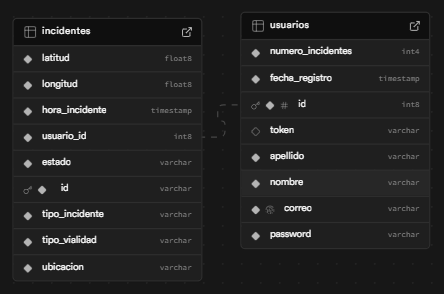
\includegraphics[scale = 1]{IMA/bd-bumper.png}
\end{center}